\documentclass{article}
\usepackage{amsmath}
\usepackage{amssymb}
\usepackage{graphicx}
\usepackage{tikz}
\usepackage{pgfplots}
\pgfplotsset{compat=1.18}
\usepackage{booktabs}
\usepackage{xcolor}

% Custom environments
\newenvironment{lesson-meta}{}{}
\newenvironment{item-analysis}{}{}
\newenvironment{model-discuss}{}{}
\newenvironment{concept-box}{}{}
\newenvironment{concept-summary}{}{}
\newenvironment{example}[1]{}{}
\newenvironment{tryit}[1]{}{}
\newenvironment{practice}[2]{}{}
\newenvironment{te-addendum}[2]{}{}
\newcommand{\answer}[1]{}
\newcommand{\placeholder}[2]{}
\newcommand{\uncertain}[2]{#1}
\newcommand{\te}[1]{}

\begin{document}

\begin{lesson-meta}
\textbf{4-3 Multiplying and Dividing Rational Expressions}

\textbf{I CAN...} find the product and the quotient of rational expressions.

\textbf{VOCABULARY}
\begin{itemize}
    \item simplified form of a rational expression
\end{itemize}

\textbf{ESSENTIAL QUESTION}
How does multiplying and dividing fractions help you multiply and divide rational expressions?
\end{lesson-meta}

\begin{model-discuss}
\textbf{EXPLORE \& REASON}

Consider the following graph of the function $y = x + 2$.

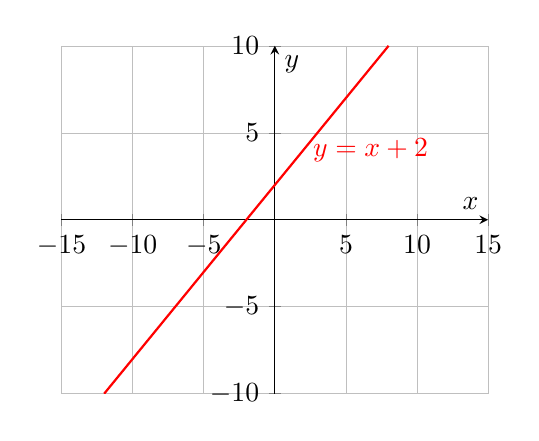
\begin{tikzpicture}
\begin{axis}[
    width=7cm, height=6cm,
    axis lines = middle,
    xmin=-15, xmax=15,
    ymin=-10, ymax=10,
    xtick={-15, -10, -5, 5, 10, 15},
    ytick={-10, -5, 5, 10},
    xlabel={$x$},
    ylabel={$y$},
    grid=both,
    grid style={line width=.1pt, draw=gray!30},
    major grid style={line width=.2pt,draw=gray!50},
]
\addplot [domain=-12:8, samples=2, color=red, thick] {x+2};
\node[red, right] at (axis cs:2, 4) {$y = x + 2$};
\end{axis}
\end{tikzpicture}

\textbf{A.} What is the domain of this function?

\textbf{B.} Sketch a function that resembles the graph, but restrict its domain to exclude 2.

\textbf{C. Use Structure} Consider the function you have sketched. What kind of function might have a graph like this? Explain.
\end{model-discuss}

\begin{concept-box}
\textbf{STUDY TIP} \\
You can make equivalent fractions by multiplying or dividing by a form of 1.
$$ \frac{4}{5} = \frac{4}{5} \cdot 1 = \frac{4}{5} \cdot \frac{2}{2} = \frac{8}{10} $$
\end{concept-box}

\begin{concept-box}
\textbf{COMMUNICATE PRECISELY} \\
A statement of equivalence between two expressions is an identity. The identity is only valid where both expressions are defined.
\end{concept-box}

\begin{example}{1}
\textbf{Write Equivalent Rational Expressions}

Write an expression that is equivalent to $\frac{x + 3}{x + 9}$. For what domain are the expressions equivalent?

You can multiply by factors of 1 in any form $\frac{a}{a}$ to write equivalent rational expressions. In this Example, multiply by $\frac{x - 6}{x - 6}$ and $\frac{x}{x}$.
$$ \frac{x + 3}{x + 9} = \frac{x + 3}{x + 9} \cdot \frac{x - 6}{x - 6} \cdot \frac{x}{x} $$
$$ = \frac{(x + 3)(x - 6)x}{(x + 9)(x - 6)x} $$
$$ = \frac{x^3 - 3x^2 - 18x}{x^3 + 3x^2 - 54x} $$

\emph{Since the denominator $x^3 + 3x^2 - 54x = x(x + 9)(x - 6)$, the expression is undefined for $0, -9$, and $6$. So the domain must exclude $0, -9$, and $6$.}

Expressions are equivalent for all values of $x$ that are in both domains. Therefore, $\frac{x + 3}{x + 9}$ is equivalent to $\frac{x^3 - 3x^2 - 18x}{x^3 + 3x^2 - 54x}$ over the domain $\{ x \mid \text{all real numbers where } x \neq 0, 6, \text{ or } -9 \}$.
\end{example}

\begin{tryit}{1}
Write an expression equivalent to $\frac{x - 4}{x}$ over the domain $\{ x \mid x \neq 0 \text{ or } -2 \}$.
\end{tryit}

\begin{concept-box}
\textbf{COMMON ERROR} \\
You may not recognize a common factor. Notice that $-1(-2 + x) = -1(x - 2)$.
\end{concept-box}

\begin{example}{2}
\textbf{Simplify a Rational Expression}

What is the simplified form of the rational expression? What is the domain for which the identity between the two expressions is valid?
$$ \frac{4 - x^2}{x^2 + 3x - 10} $$

The simplified form of a rational expression has no common factors, other than 1, in the numerator and the denominator.
$$ \frac{4 - x^2}{x^2 + 3x - 10} = \frac{(2 - x)(2 + x)}{(x - 2)(x + 5)} $$
\emph{Factor each polynomial in the numerator and denominator. The domain is all real numbers except 2 and $-5$.}
$$ = \frac{-(x - 2)(x + 2)}{(x - 2)(x + 5)} $$
\emph{Common factors divide to 1, so $\frac{-(x - 2)(x + 2)}{(x - 2)(x + 5)} = \frac{-(x - 2)}{(x - 2)} \cdot \frac{(x + 2)}{(x + 5)} = -1 \cdot \frac{(x + 2)}{(x + 5)}$.}

The simplified form of $\frac{4 - x^2}{x^2 + 3x - 10}$ is $-\frac{x + 2}{x + 5}$ for $x \neq 2$ or $-5$.
\end{example}

\begin{tryit}{2}
Simplify each expression and state the domain. \\
\textbf{a.} $\frac{x^2 + 2x + 1}{x^3 - 2x^2 - 3x}$ \qquad \textbf{b.} $\frac{x^3 + 4x^2 - x - 4}{x^2 + 3x - 4}$
\end{tryit}

\begin{concept-box}
\textbf{USE STRUCTURE} \\
Notice that the product of rational expressions is a rational expression. How can you use the definition of rational expressions to show that rational expressions are closed under multiplication?
\end{concept-box}

\begin{example}{3}
\textbf{Multiply Rational Expressions}

\textbf{A. What is the product of $\frac{2xy}{z}$ and $\frac{3x^2}{4yz}$?}

To multiply rational expressions, follow a similar method to that for multiplying two numerical fractions.
$$ \frac{2xy}{z} \cdot \frac{3x^2}{4yz} = \frac{(2xy)(3x^2)}{z(4yz)} $$
$$ = \frac{2 \cdot 3 \cdot x \cdot x^2 \cdot y}{2 \cdot 2 \cdot y \cdot z \cdot z} $$
\emph{Identify common factors that divide to 1.}
$$ = \frac{3x^3}{2z^2} $$
The product of $\frac{2xy}{z}$ and $\frac{3x^2}{4yz}$ is $\frac{3x^3}{2z^2}$ for $y \neq 0$ and $z \neq 0$.

\textbf{B. What is the product of $\frac{5x}{x + 3} \cdot \frac{x^2 + x - 6}{x^2 + 2x + 1} \cdot \frac{x^2 + x}{5x - 10}$ in simplified form?}

$$ \frac{5x}{x + 3} \cdot \frac{x^2 + x - 6}{x^2 + 2x + 1} \cdot \frac{x^2 + x}{5x - 10} = \frac{5x(x + 3)(x - 2)x(x + 1)}{(x + 3)(x + 1)(x + 1)5(x - 2)} $$
$$ = \frac{5x^2(x + 3)(x - 2)(x + 1)}{5(x + 3)(x - 2)(x + 1)(x + 1)} $$
\emph{Identify common factors that divide to 1.}
$$ = \frac{x^2}{x + 1} $$
So $\frac{5x}{x + 3} \cdot \frac{x^2 + x - 6}{x^2 + 2x + 1} \cdot \frac{x^2 + x}{5x - 10} = \frac{x^2}{x + 1}$ for $x \neq -3, -1$, or $2$.
\end{example}

\begin{tryit}{3}
Find the simplified form of each product, and state the domain. \\
\textbf{a.} $\frac{x^2 - 16}{9 - x} \cdot \frac{x^2 + x - 90}{x^2 + 14x + 40}$ \qquad \textbf{b.} $\frac{x + 3}{4x} \cdot \frac{3x - 18}{6x + 18} \cdot \frac{x^2}{4x + 12}$
\end{tryit}

\begin{concept-box}
\textbf{COMMON ERROR} \\
Only common factors, not terms, reduce to one. You cannot factor an $x$ out of $\frac{x}{x^2 + 4}$.
\end{concept-box}

\begin{example}{4}
\textbf{Multiply a Rational Expression by a Polynomial}

\textbf{What is the product of $\frac{x + 2}{x^4 - 16}$ and $x^3 + 4x^2 - 12x$?}

$$ \frac{x + 2}{x^4 - 16} \cdot (x^3 + 4x^2 - 12x) = \frac{x + 2}{x^4 - 16} \cdot \frac{x^3 + 4x^2 - 12x}{1} $$
\emph{Write 1 in the denominator to keep track of positions of factors.}
$$ = \frac{(x + 2)x(x^2 + 4x - 12)}{1(x^2 + 4)(x^2 - 4)} $$
$$ = \frac{(x + 2)x(x + 6)(x - 2)}{1(x^2 + 4)(x + 2)(x - 2)} $$
\emph{The domain is $x \neq -2$, or $2$.}

So $\frac{x + 2}{x^4 - 16} \cdot (x^3 + 4x^2 - 12x) = \frac{x(x + 6)}{x^2 + 4}$ for $x \neq -2$ or $2$.
\end{example}

\begin{tryit}{4}
Find the simplified form of each product and the domain. \\
\textbf{a.} $\frac{x^3 - 4x}{6x^2 - 13x - 5} \cdot (2x^3 - 3x^2 - 5x)$ \qquad \textbf{b.} $\frac{3x^2 + 6x}{x^2 - 49} \cdot (x^2 + 9x + 14)$
\end{tryit}

\begin{concept-box}
\textbf{USE STRUCTURE} \\
This division problem could be written as a complex fraction.
$$ \frac{\frac{x^3 + 3x^2 + 3x + 1}{1 - x^2}}{\frac{x^2 + 5x + 4}{x^2 + 3x - 4}} $$
You can rewrite any complex fraction as a division statement.
\end{concept-box}

\begin{example}{5}
\textbf{Divide Rational Expressions}

\textbf{What is the quotient of $\frac{x^3 + 3x^2 + 3x + 1}{1 - x^2}$ and $\frac{x^2 + 5x + 4}{x^2 + 3x - 4}$?}

$$ \frac{x^3 + 3x^2 + 3x + 1}{1 - x^2} \div \frac{x^2 + 5x + 4}{x^2 + 3x - 4} = \frac{x^3 + 3x^2 + 3x + 1}{1 - x^2} \cdot \frac{x^2 + 3x - 4}{x^2 + 5x + 4} $$
\emph{Multiply by the reciprocal of the divisor.}
$$ = \frac{(x + 1)(x + 1)(x + 1)(x + 4)(x - 1)}{-(x - 1)(x + 1)(x + 1)(x + 4)} $$
\emph{The domain is $x \neq -4, -1$, or $1$.}
$$ = \frac{(x + 1)}{-1} \cdot \frac{(x + 1)}{(x + 1)} \cdot \frac{(x + 1)}{(x + 1)} \cdot \frac{(x - 1)}{(x - 1)} \cdot \frac{(x + 4)}{(x + 4)} $$
$$ = -(x + 1) $$
The quotient is $-(x + 1), x \neq -4, -1$, or $1$.
\end{example}

\begin{tryit}{5}
Find the simplified quotient and the domain of each expression. \\
\textbf{a.} $\frac{1}{x^2 + 9x} \div \left( \frac{6 - x}{3x^2 - 18x} \right)$ \qquad \textbf{b.} $\frac{2x^2 - 12x}{x + 5} \div \left( \frac{x - 6}{x + 5} \right)$
\end{tryit}

\begin{concept-box}
\textbf{STUDY TIP} \\
Recall that surface area tells how much packaging material is needed and volume tells how much product the package can hold.
\end{concept-box}

\begin{example}{6}
\textbf{Use Division of Rational Expressions}

A company is evaluating two packaging options for its product line. The more efficient design will have the lesser ratio of surface area to volume. Should the company use packages that are cylinders or rectangular prisms?

\textbf{Option 1: A rectangular prism with a square base} \\
\placeholder{diagram}{Rectangular prism with length $2x$, width $2x$, and height $2x$.} \\
Surface Area: $2(2x)^2 + 4(2x)^2$ \\
Volume: $(2x)^3$

\textbf{Option 2: A cylinder with the same height as the prism, and diameter equal to the side length of the prism's base} \\
\placeholder{diagram}{Cylinder with diameter $2x$ and height $2x$.} \\
Surface Area: $2\pi x^2 + 2\pi x(2x)$ \\
Volume: $\pi x^2(2x)$

The efficiency ratio is $\frac{SA}{V}$, where $SA$ represents surface area and $V$ represents volume.

\textbf{Option 1:}
$$ \frac{SA}{V} = \frac{2(4x^2) + 4(4x^2)}{8x^3} $$
$$ = \frac{24x^2}{8x^3} $$
$$ = \frac{3}{x} $$

\textbf{Option 2:}
$$ \frac{SA}{V} = \frac{2\pi x^2 + 4\pi x^2}{2\pi x^3} $$
$$ = \frac{6\pi x^2}{2\pi x^3} $$
$$ = \frac{3}{x} $$

The company can now compare the efficiency ratio of the package designs. \\
Prism: $\frac{3}{x}$ \qquad Cylinder: $\frac{3}{x}$

In this example, the efficiency ratio of the cylinder is equal to that of the prism. So the company should choose their package design based on other criteria. \emph{Regardless of what positive value is selected for $x$, the efficiency ratios for these two package designs will be the same.}
\end{example}

\begin{tryit}{6}
The company compares the ratios of surface area to volume for two more containers. One is a rectangular prism with a square base. The other is a rectangular prism with a rectangular base. One side of the base is equal to the side length of the first container, and the other side is twice as long. The surface area of this second container is $4x^2 + 6xh$. The heights of the two containers are equal. Which has the smaller surface area-to-volume ratio?
\end{tryit}

\begin{concept-summary}
\textbf{Products and Quotients of Rational Expressions}

\begin{tabular}{lp{0.25\textwidth}p{0.25\textwidth}p{0.25\textwidth}}
\toprule
& \textbf{Multiply} & \textbf{Multiply an Integer \newline or a Polynomial} & \textbf{Divide} \\
\midrule
\textbf{RATIONAL \newline EXPRESSIONS} &
$\frac{3x}{x + 1} \cdot \frac{x^2 + x}{3x - 6}$ \newline The domain is $x \neq -1$ or $2$. &
$\frac{x + 2}{x^2 - 4} \cdot (x^2 - 2x)$ \newline $= \frac{x + 2}{x^2 - 4} \cdot \frac{x^2 - 2x}{1}$ \newline The domain is $x \neq -2$ or $2$. &
$\frac{1 - x^2}{x^2 + 3x - 4} \div \frac{x + 1}{x + 4}$ \newline $= \frac{1 - x^2}{x^2 + 3x - 4} \cdot \frac{x + 4}{x + 1}$ \newline The domain is $x \neq -4, -1$, or $1$. \\
\midrule
\textbf{WORDS} & Identify common factors and simplify. & Write the polynomial as a rational expression with 1 in the denominator. Then multiply. & Multiply by the reciprocal of the divisor. \\
\bottomrule
\end{tabular}
\end{concept-summary}

\subsection*{Do You UNDERSTAND?}

\begin{practice}{1}{1}
\textbf{ESSENTIAL QUESTION} How does multiplying and dividing fractions help you multiply and divide rational expressions?
\end{practice}

\begin{practice}{2}{1}
\textbf{Vocabulary} In your own words, define \emph{rational expression} and provide an example of a rational expression.
\end{practice}

\begin{practice}{3}{1}
\textbf{Error Analysis} A student divided the rational expressions as follows:
$$ \frac{4x}{5y} \div \frac{20x^2}{25y^2} = \frac{4x}{5y} \div \frac{5 \cdot 4x^2}{25y^2} = \frac{16x^3}{25y^3} $$
Describe and correct the errors the student made.
\end{practice}

\begin{practice}{4}{1}
\textbf{Communicate Precisely} Why do you have to state the domain when simplifying rational expressions?
\end{practice}

\subsection*{Do You KNOW HOW?}

\begin{practice}{5}{1}
What is the simplified form of the rational expression $\frac{x^2 - 36}{x^2 + 3x - 18}$? What is the domain?
\end{practice}

Find the simplified form of each product, and state the domain.

\begin{practice}{6}{1}
$\frac{4x^2y^2}{3z} \cdot \frac{15z^2}{20xy^3}$
\end{practice}

\begin{practice}{7}{1}
$\frac{y + 3}{y + 2} \cdot \frac{y^2 + 4y + 4}{y^2 - 9}$
\end{practice}

\begin{practice}{8}{1}
$\frac{x^2 + 3x - 10}{x^2 - 25} \cdot (x^2 - 9x + 20)$
\end{practice}

Find the simplified form of each quotient, and state the domain.

\begin{practice}{9}{1}
$\frac{x^3 + 14x^2 + 49x}{x^2 + 3x - 28} \div (x + 7)$
\end{practice}

\begin{practice}{10}{1}
$\frac{6x^4 + 21x^3 - 12x^2}{x^3 + x^2 - 36x - 36} \div \frac{12x^2 - 6x}{4x^2 - 144}$
\end{practice}

\subsection*{PRACTICE \& PROBLEM SOLVING}

\textbf{UNDERSTAND}

\begin{practice}{11}{1}
\textbf{Reason} Explain why $\frac{4x^2 - 7}{4x^2 - 7} = 1$ is a valid identity under the domain of all real numbers except $\pm \frac{\sqrt{7}}{2}$.
\end{practice}

\begin{practice}{12}{1}
\textbf{Error Analysis} Describe the error a student made in multiplying and simplifying
$$ \frac{x + 2}{x - 2} \cdot \frac{x^2 - 4}{x^2 + x - 2} $$
$$ = \frac{x + 2}{x - 2} \cdot \frac{x^2 - 4}{x^2 + x - 2} $$
$$ = \frac{x + 2}{x - 2} \cdot \frac{(x + 2)(x - 2)}{(x + 2)(x - 1)} $$
$$ = \frac{2}{-1} $$
\end{practice}

\begin{practice}{13}{1}
\textbf{Higher Order Thinking} Why are rational expressions closed under multiplication and division?
\end{practice}

\begin{practice}{14}{1}
\textbf{Use Appropriate Tools} Explain why domain restrictions are necessary to show that the rational expressions $\frac{-6x^2 + 21x}{3x}$ and $-2x + 7$ are equivalent. What is true about the graphs at $x = 0$ and why?
\end{practice}

\begin{practice}{15}{1}
\textbf{Generalize} Explain the similarities between rational numbers and rational expressions.
\end{practice}

\begin{practice}{16}{1}
\textbf{Use Structure} Determine whether $\frac{5x + 11}{6x + 11} = \frac{5}{6}$ is \emph{sometimes, always,} or \emph{never} true. Justify your reasoning.
\end{practice}

\begin{practice}{17}{1}
\textbf{Construct Arguments} Explain how you can tell whether a rational expression is in simplest form.
\end{practice}

\begin{practice}{18}{1}
\textbf{Communicate Precisely} When multiplying $\frac{15}{x} \cdot \frac{x}{3} = 5$, is it necessary to make the restriction $x \neq 0$? Why or why not?
\end{practice}

\begin{practice}{19}{1}
\textbf{Reason} If the denominator of a rational expression is $x^3 + 3x^2 - 10x$, what value(s) must be restricted from the domain for $x$?
\end{practice}

\textbf{PRACTICE}

Write an equivalent expression over the given domain.

\begin{practice}{20}{1}
$\frac{x(x - 2)}{(x - 5)}$ for all $x$ except $5$ and $-6$
\end{practice}

\begin{practice}{21}{1}
$\frac{3x}{x - 2}$ for all $x$ except $2$ and $-5$
\end{practice}

What is the simplified form of each rational expression? What is the domain?

\begin{practice}{22}{1}
$\frac{y^2 - 5y - 24}{y^2 + 3y}$
\end{practice}

\begin{practice}{23}{1}
$\frac{ab^3 - 9ab}{12ab^2 + 12ab - 144a}$
\end{practice}

\begin{practice}{24}{1}
$\frac{x^2 + 8x + 15}{x^2 - x - 12}$
\end{practice}

\begin{practice}{25}{1}
$\frac{x^3 + 9x^2 - 10x}{x^3 - 9x^2 - 10x}$
\end{practice}

Find the product and the domain.

\begin{practice}{26}{1}
$\frac{x^2 + 6x + 8}{x^2 + 4x + 3} \cdot \frac{x + 3}{x + 2}$
\end{practice}

\begin{practice}{27}{1}
$\frac{(x - y)^2}{x + y} \cdot \frac{3x + 3y}{x^2 - y^2}$
\end{practice}

\begin{practice}{28}{1}
$\frac{(x + 5)}{(x^3 - 25x)} \cdot (2x^3 - 11x^2 + 5x)$
\end{practice}

\begin{practice}{29}{1}
$\frac{(2x^2 - 10x)}{(x - 5)(x^2 - 1)} \cdot (3x^2 + 4x + 1)$
\end{practice}

Find the quotient and the domain.

\begin{practice}{30}{1}
$\frac{y^2 - 16}{y^2 - 10y + 25} \div \frac{3y - 12}{y^2 - 3y - 10}$
\end{practice}

\begin{practice}{31}{1}
$\frac{(x - y)^2}{x + y} \div \frac{3x + 3y}{x^2 - y^2}$
\end{practice}

\begin{practice}{32}{1}
$\frac{25x^2 - 4}{x^2 - 9} \div \frac{5x - 2}{x + 3}$
\end{practice}

\begin{practice}{33}{1}
$\frac{x^4 + x^3 - 30x^2}{x^2 - 3x - 18} \div \frac{x^3 + x^2 - 30x}{x^2 - 36}$
\end{practice}

\begin{practice}{34}{1}
Find and simplify the ratio of the volume of Figure A to the volume of Figure B.

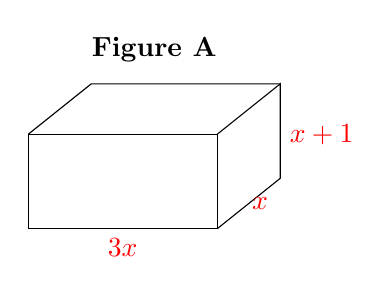
\begin{tikzpicture}[scale=0.8]
% Figure A
\draw (0,0) -- (3,0) node[midway, below, red] {$3x$} -- (3,1.5) -- (0,1.5) -- cycle;
\draw (3,0) -- (4,0.8) node[midway, right, red, inner sep=1pt] {$x$} -- (4,2.3) -- (3,1.5);
\draw (0,1.5) -- (1,2.3) -- (4,2.3);
\node[right, red] at (4,1.5) {$x+1$};
\node[above] at (2, 2.5) {\textbf{Figure A}};
\end{tikzpicture}
\qquad
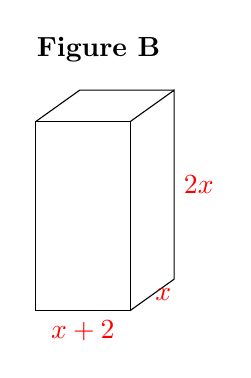
\begin{tikzpicture}[scale=0.8]
% Figure B
\draw (0,0) -- (1.5,0) node[midway, below, red] {$x+2$} -- (1.5,3) -- (0,3) -- cycle;
\draw (1.5,0) -- (2.2,0.5) node[midway, right, red, inner sep=1pt] {$x$} -- (2.2,3.5) -- (1.5,3);
\draw (0,3) -- (0.7,3.5) -- (2.2,3.5);
\node[right, red] at (2.2,2) {$2x$};
\node[above] at (1, 3.8) {\textbf{Figure B}};
\end{tikzpicture}
\end{practice}

\textbf{APPLY}

\begin{practice}{35}{1}
\textbf{Make Sense and Persevere} An engineering firm wants to construct a cylindrical structure that will maximize the volume for a given surface area. Compare the ratios of the volume to surface area of each of the cylindrical structures shown, using the following formulas for volume and surface area of cylinders.

Volume ($V$) $= \pi r^2 h$ \\
Surface Area ($SA$) $= 2\pi rh + 2\pi r^2$

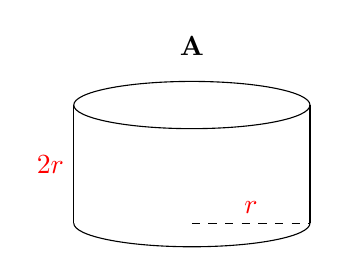
\begin{tikzpicture}
% Cylinder A
\draw (0,1.5) ellipse (1.5 and 0.3);
\draw (-1.5,0) -- (-1.5,1.5);
\draw (1.5,0) -- (1.5,1.5);
\draw (-1.5,0) arc (180:360:1.5 and 0.3);
\draw[dashed] (0,0) -- (1.5,0);
\node[above, red] at (0.75,0) {\uncertain{$r$}{$2r$}};
\node[left, red] at (-1.5,0.75) {\uncertain{$2r$}{$r$}};
\node[above] at (0, 2) {\textbf{A}};
\end{tikzpicture}
\qquad
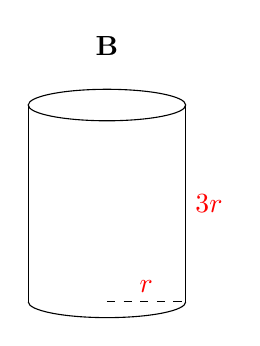
\begin{tikzpicture}
% Cylinder B
\draw (0,2.5) ellipse (1 and 0.2);
\draw (-1,0) -- (-1,2.5);
\draw (1,0) -- (1,2.5);
\draw (-1,0) arc (180:360:1 and 0.2);
\draw[dashed] (0,0) -- (1,0);
\node[above, red] at (0.5,0) {$r$};
\node[right, red] at (1,1.25) {$3r$};
\node[above] at (0, 3) {\textbf{B}};
\end{tikzpicture}

\textbf{a.} Calculate the ratio of volume to surface area for cylinder A.

\textbf{b.} Calculate the ratio of volume to surface area for cylinder B.

\textbf{c.} Which of these cylinders has a greater ratio of volume to surface area?
\end{practice}

\begin{practice}{36}{1}
\textbf{Model With Mathematics} Lupe designed a carnival game that involves tossing a beanbag into the box shown. In order to win a prize, the beanbag must fall inside the black rectangle. The probability of winning is equal to the ratio of the area of the black rectangle to the total area of the face of the box shown. Find the ratio that represents this probability in simplified form.

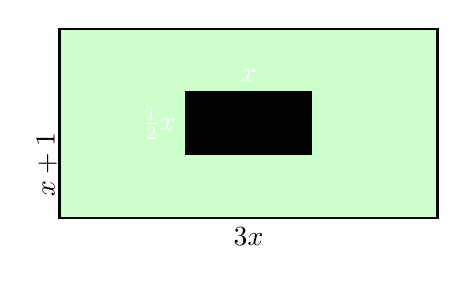
\begin{tikzpicture}[scale=0.8]
\draw[fill=green!20, draw=black, thick] (0,0) rectangle (6,3);
\draw[fill=black] (2,1) rectangle (4,2);
\node[below] at (3,0) {$3x$};
\node[left, rotate=90] at (-0.2,1.5) {$x + 1$};
\node[above, white] at (3,2) {$x$};
\node[left, white] at (2,1.5) {$\frac{1}{2}x$};
\end{tikzpicture}
\end{practice}

\begin{practice}{37}{1}
\textbf{Look for Relationships} A parallelogram with an area of $\frac{3x + 12}{10x + 25}$ square units has a height shown. Find the length of the base of the parallelogram.

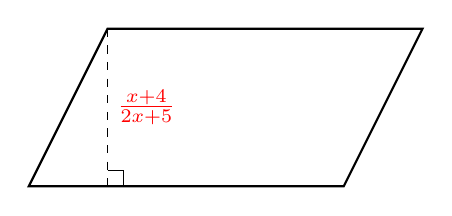
\begin{tikzpicture}
\draw[thick] (0,0) -- (4,0) -- (5,2) -- (1,2) -- cycle;
\draw[dashed] (1,2) -- (1,0);
\draw (1,0.2) -- (1.2,0.2) -- (1.2,0);
\node[right, red] at (1,1) {$\frac{x + 4}{2x + 5}$};
\end{tikzpicture}
\end{practice}

\textbf{ASSESSMENT PRACTICE}

\begin{practice}{38}{1}
Which of the following rational expressions simplify to $\frac{y}{y + 3}$? Select all that apply.
\begin{itemize}
    \item[$\square$] $\frac{(2y^2 + y)(y + 3)}{(4y + 2)(y + 3)^2}$
    \item[$\square$] $\frac{3y^2 + y}{3y^2 + 10y + 3}$
    \item[$\square$] $\frac{2y^3 + 3y^2 + y}{(2y + 1)(y^2 + 4y + 3)}$
    \item[$\square$] $\frac{y^2 + 2y}{y^2 + 4y + 3}$
    \item[$\square$] $\frac{1}{1 + \frac{3}{y}}$
\end{itemize}
\end{practice}

\begin{practice}{39}{1}
\textbf{SAT/ACT} For what value of $x$ is $\frac{2x^2 + 8x}{(x + 4)(x^2 - 9)}$ undefined? \\
A. $-8$ \\
B. $-3$ \\
C. $0$ \\
D. $4$ \\
E. $9$
\end{practice}

\begin{practice}{40}{1}
\textbf{Performance Task} The approximate annual interest rate $r$ of a monthly installment loan is given by the formula:
$$ r = \frac{\left[ \frac{24(nm - p)}{n} \right]}{\left( p + \frac{nm}{12} \right)} $$
where $n$ is the total number of payments, $m$ is the monthly payment, and $p$ is the amount financed.

\textbf{Part A} Find the approximate annual interest rate (to the nearest percent) for a four-year signature loan of $\$20,000$ that has monthly payments of $\$500$.

\textbf{Part B} Find the approximate annual interest rate (to the nearest tenth percent) for a five-year auto loan of $\$40,000$ that has monthly payments of $\$750$.
\end{practice}

\end{document}
